\documentclass[german,10pt]{article}
\usepackage[a4paper, margin={3cm}]{geometry}
\usepackage[utf8]{inputenc}
\usepackage[T1]{fontenc}
\usepackage{makecell}
\usepackage{lastpage}
\usepackage{fancyhdr}
\usepackage{graphicx}
\pagestyle{fancy}
\title{Curriculum Vitae}
\author{Tobias Hochreiter}
\date{}
\begin{document}
	\cfoot{\thepage\ / \pageref*{LastPage}}
	\vspace*{-1.5cm}
	%\hrule
	\begin{picture}(0,0)
		\put(300,-160){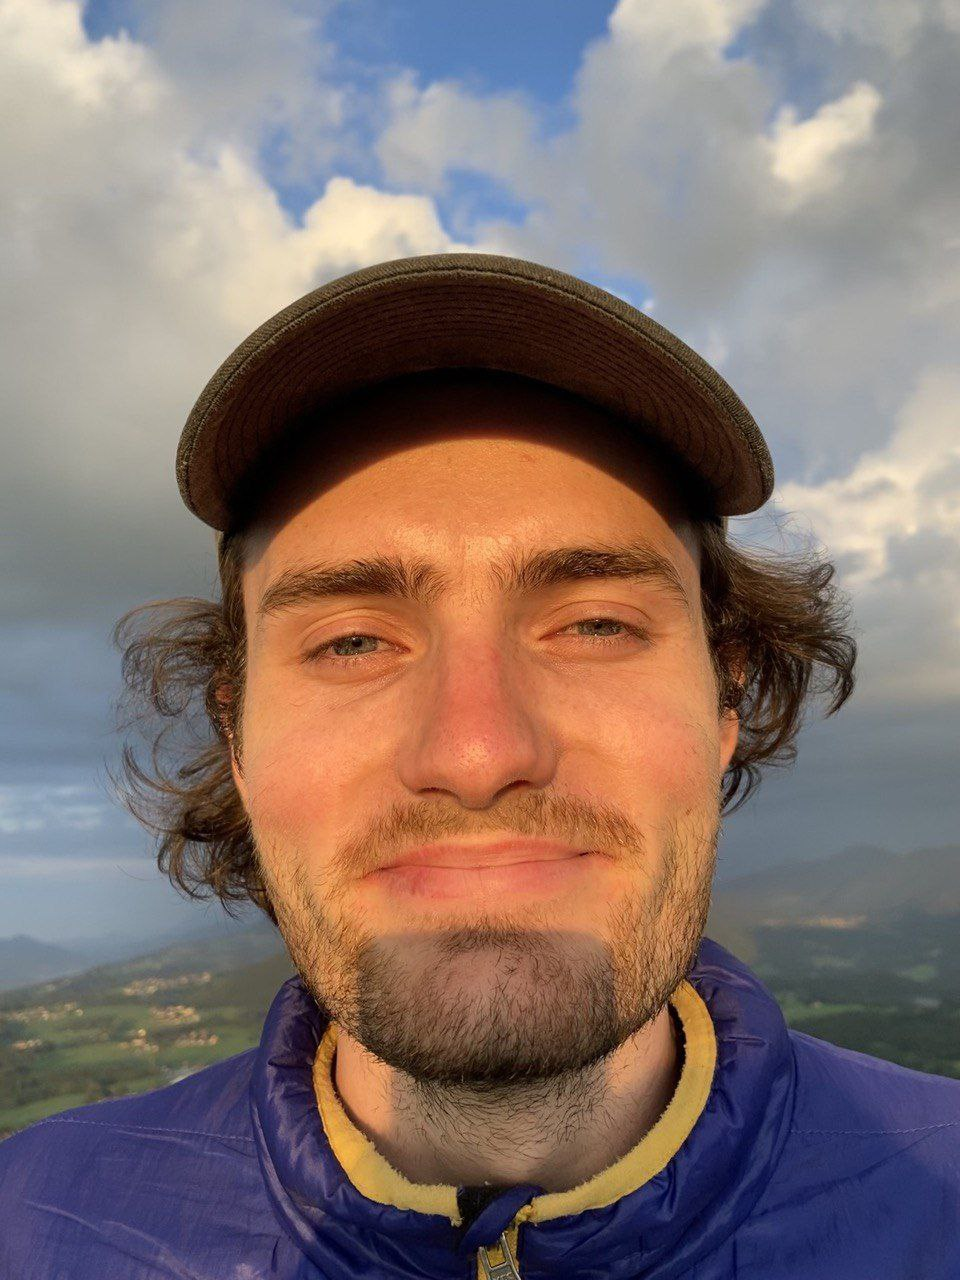
\includegraphics[width=3.5cm]{../moi1.jpg}}
	\end{picture}
	\begin{center}
		\textbf{\LARGE Curriculum Vitae}\\
		\vspace{.4cm}
		{\large Tobias Hochreiter}\\
		\vspace{.2cm}
		tobias.hochreiter@gmx.at
	\end{center}
	\section*{Persönliche Daten}
	geboren am 10/10/1997 in Salzburg, Österreich\\
	österreichischer Staatsbürger\\
	ledig
	
	\section*{Bildung}
	\begin{tabular}{m{3cm}|l}
		04/2021 - 06/2023 & \makecell{\textbf{UHH} (Hamburg): M.Sc. Mathematische Physik ($1.0$, s.c.l.)\\\textit{Über Topologische Quantenfeldtheorien}}\\[9pt]
		10/2017 - 06/2021 & \makecell{\textbf{TUM} (Munich): B.Sc. Physik ($1.3$, c.l.)\\\textit{Physikalische und Geometrische Aspekte der Korteweg de Vries Gleichung}}\\[9pt]
		09/2011 - 05/2016 & HTL Salzburg: Oberstufe BHS, Abt. \textit{Gesundheitstechnik} ($1.4$, s.c.l.)\\
		09/2007 - 07/2011 & Werkschulheim Felbertal: Internat mit Schwerpunkt auf Handwerk
	\end{tabular}
	
	\section*{Zivildienst}
	\begin{tabular}{m{3cm}|l}
		08/2016 - 04/2017 & Sanitäter \& Fahrer für das Rote Kreuz Salzburg
	\end{tabular}
	
	\section*{Praktika}
	\begin{tabular}{m{3cm}|l}
		\makecell{Sommer 2017\\(12 Wochen)} & AB Mikroelektronik (Platinenplanung und -fertigung, C++ Programmierung)\\
		\makecell{Sommer 2014\\(4 Wochen)} & AML Elektrotechnik (Elektroinstallationen am Bau)\\
		\makecell{Sommer 2013\\(4 Wochen)} & SALK (Krankenhaus, Aushilfe in der Abt. \textit{Medizintechnik})
	\end{tabular}
	
	\section*{Nebenberufe}
	\begin{tabular}{m{3cm}|l}
		10/2022 - 03/2023 & Tutor: \textit{Analysis 3 für Physiker} (unterrichten, verbessern)\\
		10/2020 - 03/2021 & Tutor: \textit{Theoretische Physik, stat. Mech.} (unterrichten, verbessern, unterstützen)\\
		04/2020 - 09/2020 & Tutor: \textit{Theoretische Physik, QM} (unterrichten, verbessern, unterstützen)\\
		10/2019 - 03/2020 & Tutor: \textit{Theoretische Physik, Edyn.} (unterrichten, verbessern, unterstützen)\\
		04/2019 - 09/2019 & Tutor: \textit{Theoretische Physik, klass. Mech.} (unterrichten, verbessern, unterstützen)\\
		12/2014 - 04/2017 & IB-Krallinger (Planung für Elektroinstallationen am Bau)\\
		10/2013 - 07/2014 & AML Elektrotechnik (Elektroinstallateur, Schaltkästenbau)
	\end{tabular}
	
	\section*{Stipendien}
	\begin{tabular}{m{3cm}|l}
		10/2018 - 10/2023 & Max Weber-Programm Bayern (Begabtenförderung à 215€/Monat)
	\end{tabular}
	
	\section*{Sprachen}
	\begin{tabular}{m{3cm} | l}
		Deutsch & Muttersprache\\
		Englisch & Niveau ca. C1 (aus Studium)\\
		Französisch & Niveau B2 von \textit{DELF}-Prüfung\\
		&
	\end{tabular}
	\hrule
\end{document}